\documentclass[border=2pt]{standalone}
\usepackage{circuitikz}
\ctikzset{capacitors/width=.25}
\begin{document}
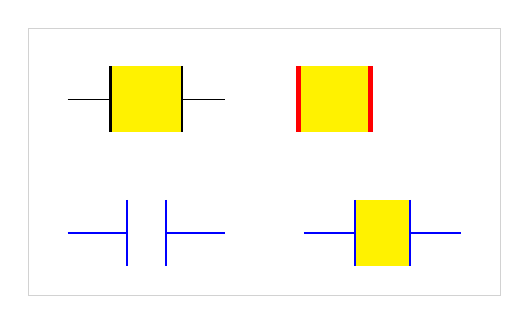
\begin{tikzpicture}[circuitikz/capacitors/width=.35]
  \draw[gray!35] (-.5,-.8) rectangle (5.5,2.6);
  \draw[blue] (0,0) to[C] (2,0);
  \ctikzset{capacitors/width=.5,capacitors/fill=yellow}
  \begin{scope}[circuitikz/capacitors/width=.65]
    \draw[red,thick] (3.3,1.7) to[C] (3.48,1.7);
    \draw (0,1.7) to[C,fill=none] (2,1.7);
  \end{scope}
  \draw[blue] (3,0) to[C] (5,0);
\end{tikzpicture}
\end{document}
